\documentclass[]{scrreprt}
\usepackage{amsmath,amsfonts,graphicx}
%\usepackage{multirow}
%\usepackage{pslatex}
%\usepackage{tabularx}
%\usepackage{comment}
%\usepackage{xspace}
%\usepackage{array}

%\usepackage{hyperref}

%\usepackage{caption}
%\DeclareCaptionFont{white}{\color{white}}
%\DeclareCaptionFormat{listing}{\colorbox{gray}{\parbox{\textwidth}{#1#2#3}}}

\def\species{\mathrm{sp}}
\def\phase{\mathrm{ph}}
\def\massfrac{\chi}
\def\flux{\mathbf{F}}
\def\darcyvel{\mathbf{v}}
\def\energydens{\mathcal{E}}
\def\d{\mathrm{d}}

\newcommand{\uo}{\mbox{UO\textsubscript{2}}\xspace}

\setcounter{secnumdepth}{3}


\begin{document}


\title{Heat Advection Tests}
\author{CSIRO}
\maketitle

\tableofcontents

\chapter{One-dimensional heat advection via a single-phase fluid}

Consider the case of a single-phase fluid in 1 dimension, $0\leq x
\leq 1$, with the porepressure fixed at the boundaries:
\begin{equation}
P(x=0, t) = 1 \ \ \ \mbox{and}\ \ \ P(x=1, t) = 0 \ .
\end{equation}
With zero gravity, and high fluid bulk modulus, the Darcy equation
implies that the solution is $P(x, t) = 1 - x$, with
\begin{equation}
v = k/\mu
\end{equation}
being the constant\footnote{To get the velocity of the individual
  fluid particles, this should be divided by the porosity.} ``Darcy
velocity'' from $x=0$ to $x=1$.  Here $k$ is the porous medium's
permeability, and $\mu$ is the fluid dynamic viscosity.

Suppose that the fluid internal energy is given by $CT$, where $C$ is
the specific heat capacity and $T$ is its temperature.  Assuming that
$P/\rho \ll CT$, then the fluid's enthalpy is also $CT$.  In this
case, the energy equation reads
\begin{equation}
\left((1 - \phi)\rho_{R}C_{R} + \phi\rho C \right) \frac{\partial
  T}{\partial t} + C \rho v \frac{\partial T}{\partial x} = 0 \ .
\end{equation}
This is the wave equation with velocity
\begin{equation}
v_{T} = \frac{C\rho v}{(1 - \phi)\rho_{R}C_{R} + \phi\rho C} \ .
\end{equation}
Recall that the ``Darcy velocity'' is $v=k/\mu$.

Let the initial condition for $T$ be $T(x, t=0) = 200$.  Apply the
boundary conditions
\begin{equation}
T(x=0, t) = 300 \ \ \ \mbox{and} \ \ \ T(x=1, t) = 200 \ .
\end{equation}
At $t=0$ this creates a front at $x=0$.  Choose the parameters $C=2$,
$C_{R}=1$, $\rho=1000$, $\rho_{R}=125$, $\phi=0.2$, $k=1.1$, $\mu=4.4$
(all in consistent units), so that $v_{T}=1$ is the front's velocity.

The sharp front is {\em not} maintained by
MOOSE.  This is due to numerical diffusion, which is particularly
strong in the upwinding scheme implemented in the PorousFlow module.
Nevertheless, MOOSE advects the smooth front with the correct
velocity, as shown in Figure~\ref{heat_advection_1d.fig}.

\begin{figure}[htb]
\begin{center}
\begin{tabular}{cc}
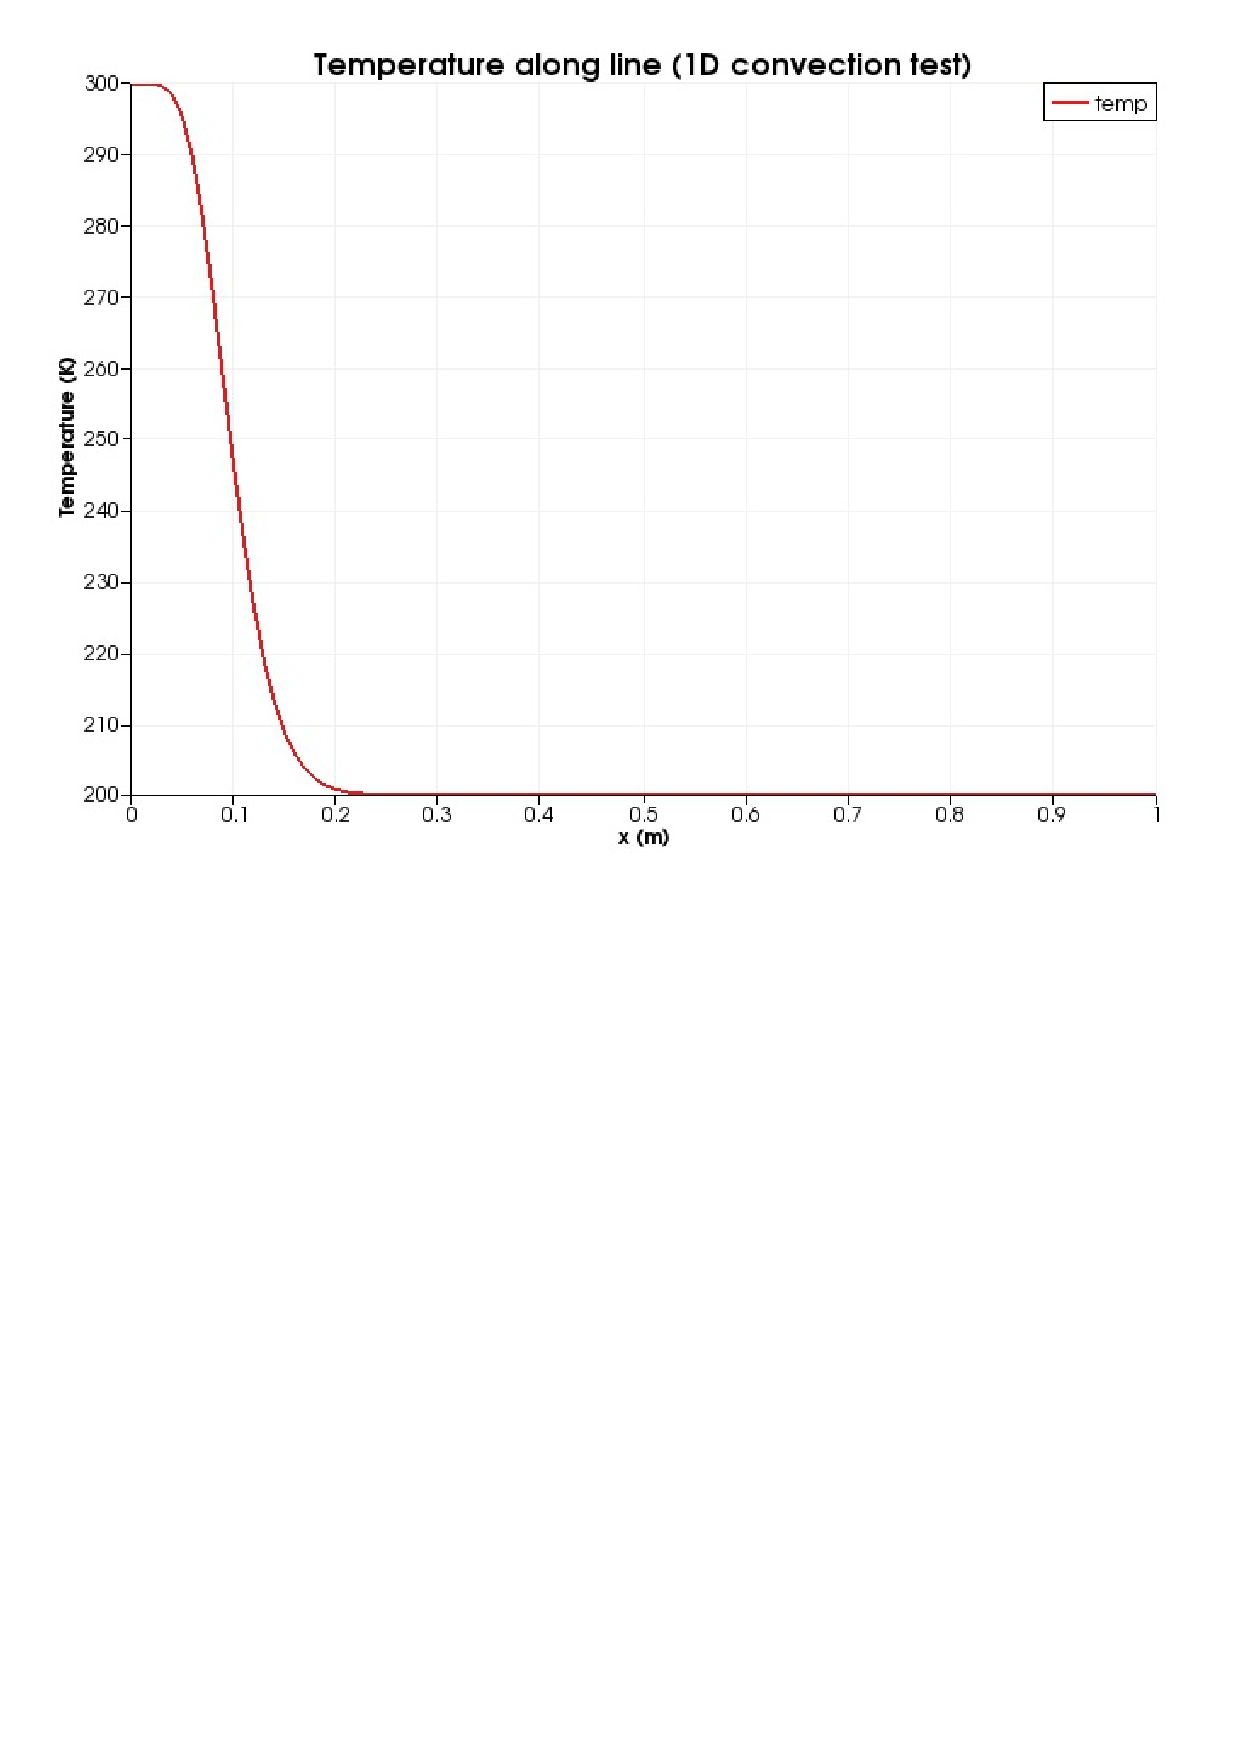
\includegraphics[width=7cm]{heat_advection_1d_0_1.pdf}  &
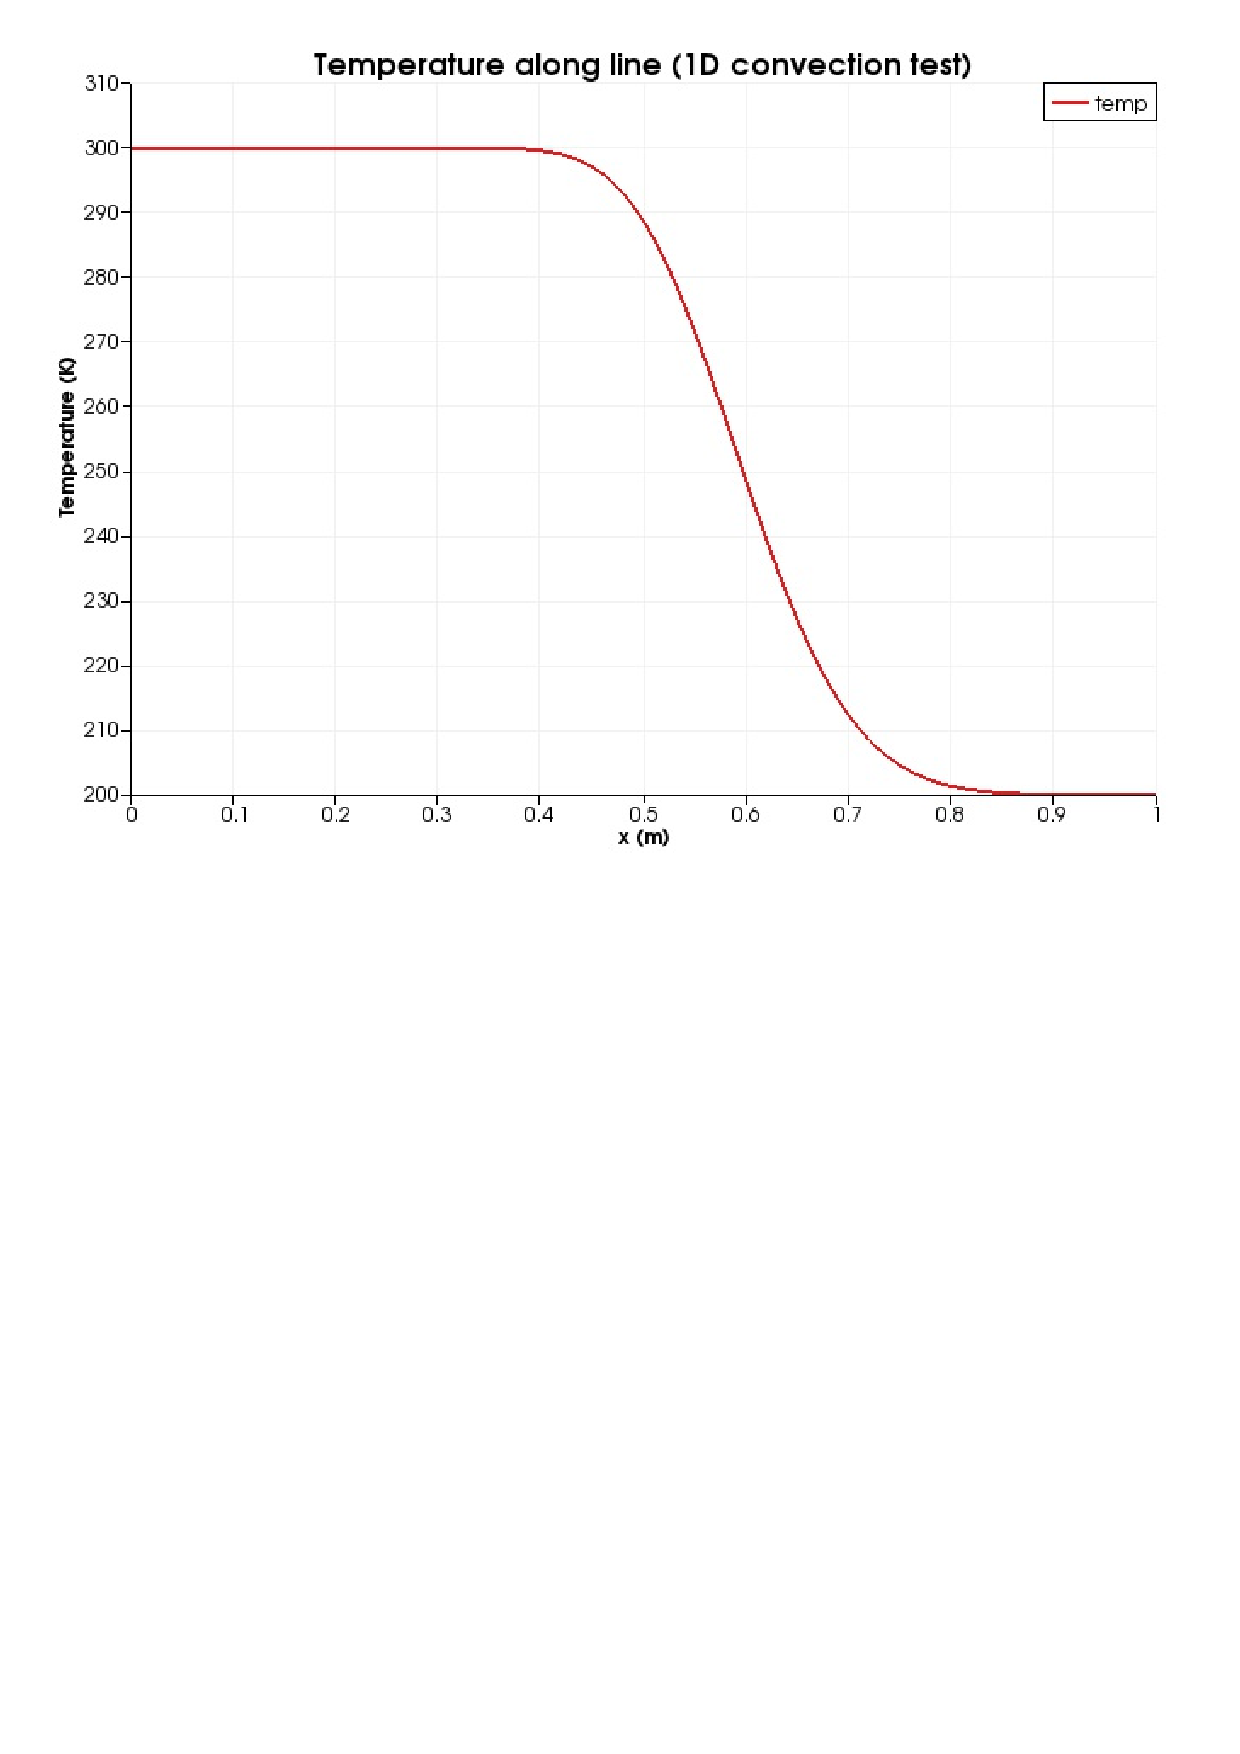
\includegraphics[width=7cm]{heat_advection_1d_0_6.pdf}
\end{tabular}
\caption{Results of heat advection via a fluid in 1D.  The fluid
  flows with constant Darcy velocity of $0.25$\,m.s$^{-1}$ to the
  right, and this advects a temperature front at velocity
  $1$\,m.s$^{-1}$ to the right.  This pictures above
  that the numerical implementation of porous flow within
  MOOSE diffuses sharp fronts, but advects them at the correct
  velocity (notice the centre of
  the front is at the correct position in each picture).  Left: temperature
  $t=0.1$\,s.  Right: temperature
  at $t=0.6$\,s.}
\label{heat_advection_1d.fig}
\end{center}
\end{figure}







\end{document}

